\documentclass[uplatex,a4j,11pt,dvipdfmx]{jsarticle}
\usepackage{listings,jvlisting}
\bibliographystyle{junsrt}

\usepackage{url}

\usepackage{graphicx}
\usepackage{gnuplot-lua-tikz}
\usepackage{pgfplots}
\usepackage{tikz}
\usepackage{amsmath,amsfonts,amssymb}
\usepackage{bm}
\usepackage{siunitx}

\makeatletter
\def\fgcaption{\def\@captype{figure}\caption}
\makeatother
\newcommand{\setsections}[3]{
\setcounter{section}{#1}
\setcounter{subsection}{#2}
\setcounter{subsubsection}{#3}
}
\newcommand{\mfig}[3][width=15cm]{
\begin{center}
\includegraphics[#1]{#2}
\fgcaption{#3 \label{fig:#2}}
\end{center}
}
\newcommand{\gnu}[2]{
\begin{figure}[hptb]
\begin{center}
\input{#2}
\caption{#1}
\label{fig:#2}
\end{center}
\end{figure}
}

\begin{document}
\title{応用プラズマ工学}
\author{82311971 佐々木良輔}
\date{}
\maketitle
\subsection*{(1)}
エネルギー保存則
\begin{align}
  \frac{1}{2}m_iv_x^2+Ze\phi=0
\end{align}
ポアソン方程式
\begin{align}
  \frac{d^2\phi}{dx^2}=-\frac{\rho}{\varepsilon_0}
\end{align}
電流連続の式
\begin{align}
  j(x)=\rho(x)v_x(x)={\rm const.}
\end{align}
\subsection*{(2)}
(1)式を$v_x$について解くと
\begin{align}
  \everymath{\displaystyle}
  \begin{array}{cc}
    &v_x^2=-\frac{2Ze\phi(x)}{m_i}\\
    \therefore&v_x=\sqrt{-\frac{2Ze\phi(x)}{m_i}}
  \end{array}
\end{align}
また(3)式において$j(x)$が一定であることから$j(x)=j_0$と置くと
\begin{align}
  \everymath{\displaystyle}
  \begin{array}{cc}
    &j_0=\rho(x)\sqrt{-\frac{2Ze\phi(x)}{m_i}}\\
    \therefore&\rho(x)=\frac{j_0}{\sqrt{-\frac{2Ze\phi(x)}{m_i}}}
  \end{array}
\end{align}
これを(2)式に代入すれば
\begin{align}
  \frac{d^2\phi}{dx^2}=-\frac{j_0}{\varepsilon_0\sqrt{-\frac{2Ze\phi(x)}{m_i}}}
\end{align}
を得る.ここで$x=X\delta$, $\phi=-\Phi V$と変数変換すると
\begin{align}
  \everymath{\displaystyle}
  \begin{array}{cc}
    &\frac{d^2(-\Phi V)}{d(X\delta)^2}=-\frac{j_0\sqrt{m_i}}{\varepsilon_0\sqrt{-2Ze(-\Phi V)}}\\
    \iff&-\frac{V}{\delta^2}\frac{d^2\Phi}{dX^2}=-\frac{j_0\sqrt{m_i}}{\varepsilon_0\sqrt{2ZeV}}\Phi^{-1/2}\\
    \iff&\frac{d^2\Phi}{dX^2}=\frac{j_0}{\varepsilon_0}\sqrt{\frac{m_i}{2Ze}}\frac{\delta^2}{V^{3/2}}\Phi^{-1/2}\\
    \iff&\frac{d^2\Phi}{dX^2}=\alpha\Phi^{-1/2}
  \end{array}
\end{align}
を得る.
\subsection*{(3)}
(7)の両辺に$2\Phi'$を乗ずると
\begin{align}
  2\Phi'\Phi''=2\alpha\Phi'\Phi^{-1/2}
\end{align}
ここで
\begin{align}
  \frac{d}{dX}(\Phi'(X))^2=2\Phi'(X)\frac{d}{dX}\Phi'(X)\\
  2\frac{d}{dX}(\Phi(X))^{1/2}=2\times\frac{1}{2}\Phi(X)\frac{d}{dX}\Phi(X)
\end{align}
なので(8)式は
\begin{align}
  \frac{d}{dX}(\Phi'(X))^2=4\alpha\frac{d}{dX}(\Phi(X))^{1/2}
\end{align}
これを両辺$X\in[0,X]$で積分すると
\begin{align}
  \begin{split}
    \int_{0}^{X}\frac{d}{dX}(\Phi'(X))^2dX&=\int_{0}^{X}4\alpha\frac{d}{dX}(\Phi(X))^{1/2}dX\\
    \Bigl[(\Phi'(X))^2\Bigr]_0^X&=4\alpha\Bigl[(\Phi(X))^{1/2}\Bigr]_0^X\\
    (\Phi'(X))^2-(\Phi'(0))^2&=4\alpha\left((\Phi(X))^{1/2}-(\Phi(0))^{1/2}\right)
  \end{split}
\end{align}
ここで境界条件$\Phi'(0)=\Phi(0)=0$から
\begin{align}
  \everymath{\displaystyle}
  \begin{array}{cc}
    &(\Phi'(X))^2=4\alpha(\Phi(X))^{1/2}\\
    \iff&\Phi'(X)=2\sqrt{\alpha}(\Phi(x))^{1/4}\\
    \iff&\frac{d\Phi(X)}{(\Phi(X))^{1/4}}=2\sqrt{\alpha}dX
  \end{array}
\end{align}
これは変数分離形なので, 両辺を積分すると
\begin{align}
  \everymath{\displaystyle}
  \begin{array}{cc}
    &\int_{0}^{\Phi}\frac{d\Phi(X)}{(\Phi(X))^{1/4}}=2\sqrt{\alpha}\int_{0}^{X}dX\\
    \iff&\left[\frac{4}{3}(\Phi(X))^{3/4}\right]_0^\Phi=2\sqrt{\alpha}X
  \end{array}
\end{align}
境界条件から
\begin{align}
  \frac{4}{3}(\Phi(X))^{3/4}=2\sqrt{\alpha}X
\end{align}
また境界条件$\Phi(X)|_{X=1}=1$から
\begin{align}
  \frac{4}{3}=2\sqrt{\alpha}
\end{align}
以上から
\begin{align}
  \everymath{\displaystyle}
  \begin{array}{cc}
    &(\Phi(X))^{3/4}=X\\
    \iff&\Phi(X)=X^{4/3}\\
    \iff&-\frac{\phi(x)}{V}=\left(\frac{x}{d}\right)^{4/3}\\
    \iff&\phi(x)=-V\left(\frac{x}{d}\right)^{4/3}
  \end{array}
\end{align}
を得る.
\subsection*{(4)}
$\phi(x)$は図1のようなグラフになる.ただし$d=3$, $V=2$としてプロットした.
プラズマが存在しないとき,電位は線形の勾配を持つが,ここでは$x\simeq0$でより緩やかな勾配になっている.
これはプラズマ粒子が存在することにより電場の遮蔽が起きたことによるものである.
$x>0$でのプラズマ密度が平衡状態より多くなると, $x\simeq0$での電位勾配が正になるためプラズマ粒子は$x>0$の領域へ出にくくなる,
逆に$x>0$でのプラズマ密度が平衡状態より少なくなると, 電位勾配が負になるためプラズマ粒子が$x>0$へ出やすくなる.
このようなフィードバックがかかるため,電荷制限電流が生じる.
\begin{center}
  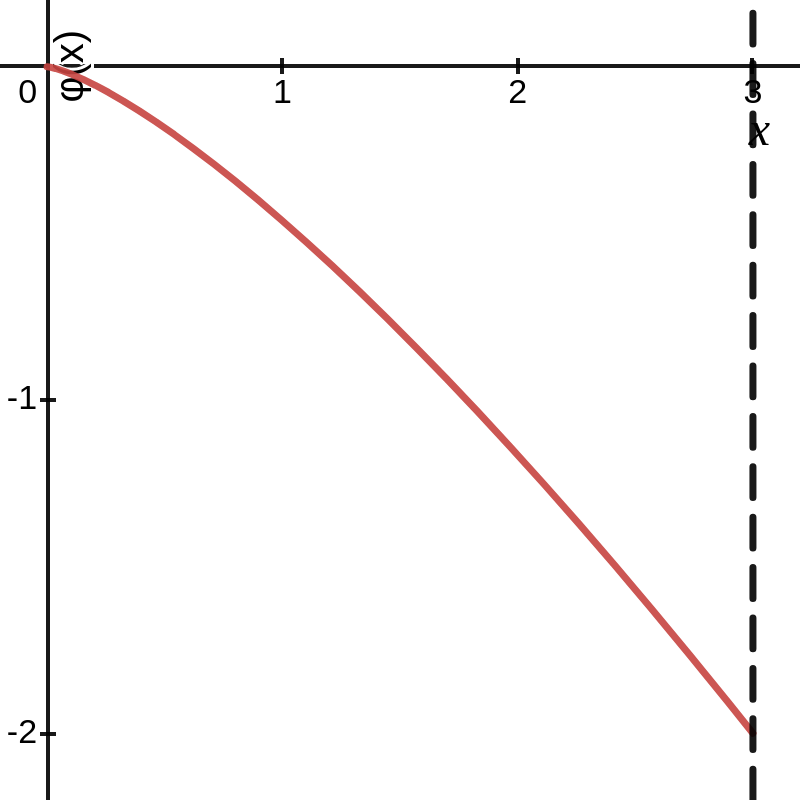
\includegraphics[width=6cm]{x-phi.png}
  \fgcaption{$\phi(x)$のグラフ}
\end{center}
\subsection*{(5)}
(7)式から
\begin{align}
  \alpha=\frac{j_0}{\varepsilon_0}\sqrt{\frac{m_i}{2Ze}}\frac{\delta^2}{V^{3/2}}
\end{align}
また(16)式から$\alpha=4/9$なので
\begin{align}
  \everymath{\displaystyle}
  \begin{array}{cc}
    &\frac{j_0}{\varepsilon_0}\sqrt{\frac{m_i}{2Ze}}\frac{\delta^2}{V^{3/2}}=\frac{4}{9}\\
    \iff&j_0=\frac{4}{9}\varepsilon_0\sqrt{\frac{2Ze}{m_i}}\frac{V^{3/2}}{\delta^2}
  \end{array}
\end{align}
を得る.
\subsection*{(6)}
(19)式からArプラズマと水素プラズマで同量の電流を得るには
\begin{align}
  \everymath{\displaystyle}
  \begin{array}{cc}
    &\frac{4}{9}\varepsilon_0\sqrt{\frac{2Z_{\rm H_2}e}{m_{\rm H_2}}}\frac{V_{\rm H_2}^{3/2}}{\delta^2}
    =\frac{4}{9}\varepsilon_0\sqrt{\frac{2Z_{\rm Ar}e}{m_{\rm Ar}}}\frac{V_{\rm Ar}^{3/2}}{\delta^2}\\
    \iff&\frac{V_{\rm Ar}^{3/2}}{V_{\rm H_2}^{3/2}}=\sqrt{\frac{m_{\rm Ar}}{m_{\rm H_2}}}\\
    \iff&\frac{V_{\rm Ar}}{V_{\rm H_2}}=\left(\frac{m_{\rm Ar}}{m_{\rm H_2}}\right)^{1/3}
  \end{array}
\end{align}
ただし$Z_{\rm H_2}=Z_{\rm Ar}$を用いた.ここで質量比は原子量比と考えて良く, Arの原子量は40, 水素の原子量は1であるので,
\begin{align}
  \frac{V_{\rm Ar}}{V_{\rm H_2}}=\left(\frac{40}{1}\right)^{1/3}\simeq3.4
\end{align}
となる.
\end{document}